\documentclass[cn,11pt]{elegantbook}
%-------------------------------------------
%-------------------------------------------
% 只检查错误,不编译,提高速度
%\usepackage{syntonly}
%\syntaxonly %只编译
%-------------------------------------------
%-------------------------------------------
% 只显示部分内容
%\includeonly{6}
%-------------------------------------------
%-------------------------------------------
% MATLAB
\usepackage{matlab-prettifier}%matlab排版
\usepackage[T1]{fontenc}%matlab字体

\usepackage{siunitx,physics}

%\setCJKmainfont{微软雅黑}  %中文字体设置
%\setCJKsansfont{楷体} %设置中文字体
%\setCJKmonofont{} %设置中文字体

\lstset{style=Matlab-editor,
  escapechar=`,
  frame=shadowbox,
  numbers=none
} % 定义默认代码块格式
%-------------------------------------------
%-------------------------------------------、
% 封面页设置
\title{《化工数值计算与MATLAB》复习指南}
\subtitle{——计算机化工应用\ ||\ \href{https://github.com/WsinGithub/ChemEngMATLAB}{ChemEngMATLAB}}
\author{王世强}
\institute{华东理工大学化工学院}
\date{\today}
\version{0.4\ ||\ 本文模板来自\href{https://elegantlatex.org/}{Elegant\LaTeX{} 项目组}}
\extrainfo{}
\logo{logo.png}
\cover{cover.png}
\extrainfo{注:封面图选自《日常》第零集}
%-------------------------------------------
%-------------------------------------------
\begin{document}
% 标题页开关
\maketitle \tableofcontents 
%\thispagestyle{empty}
\mainmatter
\hypersetup{pageanchor=true}
%-------------------------------------------
\chapter*{写在前面\footnote{点击目录后的页码可快速跳转到指定内容,也可以在书签页快速浏览。}}
期末临近,本文将作为华理化工学院专业必修课程“计算机化工应用”的复习指南。

本文制作过程中主要参考了隋志军老师的教材《化工数值计算与MATLAB》、作业、课件,并参考了付金硕学长的相关资料。在文档制作过程中还得到了\LaTeX{}技术交流 1 群与\LaTeX{}科技排版工作室中网(da)友(lao)们的帮助,在此感谢他们!
\begin{lstlisting}[frame=single,numbers=left]
% 此环境下主要介绍函数的写法
其中,`\mlplaceholder{空缺}`通常表示占位符。
while `\mlplaceholder{condition}`
    if `\mlplaceholder{something-happens}`
        % do something useful
    end
end
\end{lstlisting}

\begin{lstlisting}
% 此环境下主要给出例题的解答,各位可以直接复制到MATLAB中运行
function exam5_3_1
t=3:3:30;
G1=[10.2 13.9 12.16 13.49 13.74 12.01 11.55 11.02 12 12.12];
G2=[6.91 8.94 8.69 10.09 10.63 9.58 9.53 9.29 10.13 10.24];
A=1.83;
X=(G1-G2)./G2;
tt=linspace(3,30);
% 插值
pp=spline(t,X);
ppv=-fnval(pp,tt)/A;
% 微分
dp=fnder(pp);dpv=fnval(dp,tt);
plot(t,X,'ro',tt,ppv,tt,dpv,'.-')
axisX=refline(0,0)
axisX.Color='c'
legend('原始数据','拟合曲线','导数曲线','导数参考直线')
\end{lstlisting}

时间仓促,错误\footnote{各位如果发现写错的地方,请联系我QQ568365675!}与疏漏\footnote{后续更新于\href{https://github.com/WsinGithub/ChemEngMATLAB}{https://github.com/WsinGithub/ChemEngMATLAB}}在所难免,请各位辩证地使用!

最后,预祝各位期末顺利,门门4.0!

\chapter*{绪论部分}
\addcontentsline{toc}{chapter}{绪论部分}
\markboth{绪论部分}{}
\begin{introduction}
\item 误差
\item 浮点数及其运算
\item MATLAB 的常用命令
\end{introduction}
\section{误差}
\subsection{误差来源}
\begin{itemize}
  \item \textbf{模型误差},问题简化过程产生
  \item \textbf{截断误差},有限次运算限制产生
  \item \textbf{舍入误差},机器字长限制产生
\end{itemize}
有关误差定义不再赘述,举Work1中一例:
\begin{problem}
已知某化工管道的真实长度为 1000m,某次测量结果为 1001m,其测量的绝
对误差,相对误差为多少?
\end{problem}

\begin{solution}
绝对误差为 1m,相对误差为 0.1\%。
\end{solution}

\section{浮点数与浮点数运算}
\subsection{浮点数}
由于计算机资源的有限,在计算机上只能表示有限的实数,这些数被称为浮点数。

浮点数有如下性质:\textbf{有限个、有界、非连续。}
\subsection{IEEE标准双精度浮点运算体系}

\begin{definition}{特殊浮点数}{}
最大实数(上溢:超过用inf或Inf表示):
\[real_{max}=1.79e+308
\]
最小正实数(下溢:若为小于其的正数,则记为0):
\[real_{min}=2.225e-308
\]
从1到下一个较大浮点数的距离(机器精度):
\[eps=2^{-52}=2.220e-16
\]
\end{definition}
\subsection{浮点数运算}
浮点数运算,加法和乘法运算交换律仍然适用,但是
其结合律和分配律已不再适用。
\begin{definition}{NaN}{}
 Not a Number,非数。
\end{definition}

计算下列情况时会出现,

\begin{itemize}
  \item 0 / 0
  \item $\infty / \infty$
  \item (+Inf) + (-Inf)
  \item 0 * Inf
\end{itemize}
\section{MATLAB的通用命令}
\begin{definition}{常用命令}{}
 clc:清除命令窗口内容
 
 clear:清除内存变量
 
 save:保存内存变量到指定文件
\end{definition}

\begin{lstlisting}[frame=single,numbers=left]
clc,clear %通常用作初始化
\end{lstlisting}
\chapter{MATLAB程序设计语言与初等数学运算}
\begin{introduction}
\item 变量与数据类型
\item 数据~/~图形输出
\item 逻辑运算
\item 函数
\item 控制语句
\end{introduction}

\begin{note}
本章内容较繁杂,仅列举考试主体,细节请各位自行翻阅课本及课件!
\end{note}

\section{变量与数据}
\subsection{变量与数据}
\begin{itemize}
  \item 命名规则
  \item 常用变量
\end{itemize}
\subsection{数据类型}
\begin{itemize}
  \item 数值(向量、矩阵,用~[]~标识,注意区分~,~~/~~\verb*+ +与~;~)
  \item 字符(用'\mlplaceholder{string}'标识)
  \item 单元数组,cell array(注意'\{\}'的使用方法)
  \item 结构体,structure(用'.'标识)
  \item 函数句柄
\end{itemize}
\subsection{生成向量}
\begin{lstlisting}[frame=single,numbers=left]
a=1:10 %默认以1为间距
a=1:2:10 %以2为间距
% 线性等分
y=linspace(`\mlplaceholder{start}`,`\mlplaceholder{end}`(,`\mlplaceholder{n}`))
% 对数等分
y=logspace(`\mlplaceholder{start}`,`\mlplaceholder{end}`(,`\mlplaceholder{n}`))
\end{lstlisting}
\newpage
\section{数据输出}
\subsection{disp函数}
\begin{lstlisting}[frame=single,numbers=left]
%显示`\mlplaceholder{X}`到屏幕,并自动换行
disp(`\mlplaceholder{X}`)
% 输出矩阵
a=[1 2;3 4];
disp(a)
% 输出字符
disp('A') %将输出字母A
disp(['1+1=',num2str(2)]) %使用 [] 连接字符
\end{lstlisting}

\subsection{fprintf函数}

\begin{definition}{常用转义字符}{}
\%n~换行~~~\%t制表符~~~\%f固定位数小数~~~\%s~字符或字符串~~~\%e~指数形式
\end{definition}
举例如下:
\begin{lstlisting}
% Work2_4 计算压降
L=3000;d=45;V=1600;
deltP=0.03*L*(V/1000)^1.84/d^1.24;
disp('L=3000m d=45mm V=1600m/min')
disp('压降计算值为:')
fprintf('\tdeltP=%.2e\n',deltP)
\end{lstlisting}
\begin{figure}[htbp]
	\centering
	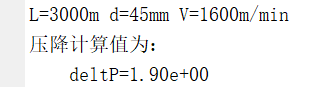
\includegraphics[width=0.6\textwidth]{fprintf.png}
	\caption{运行结果}
\end{figure}
\newpage
\section{图形输出}
\subsection{基本概念}
\begin{lstlisting}[frame=single,numbers=left]
% 可将多条曲线绘制于同一图形窗口
% '`\mlplaceholder{S}`'对线型、颜色、数据点形貌等设置
% 线型 -实线  :虚线  -.点划线 --双画线
% 颜色 b蓝色 g绿色 r红色 k黑色
% 点貌 .黑心实点 o空心圆圈 p五角星符
plot(`\mlplaceholder{X1}`,`\mlplaceholder{Y1}`,'`\mlplaceholder{S1}`',`\mlplaceholder{X2}`,`\mlplaceholder{Y2}`,'`\mlplaceholder{S2}`',…)
\end{lstlisting}
示例如下:
\begin{figure}[htbp]
	\centering
	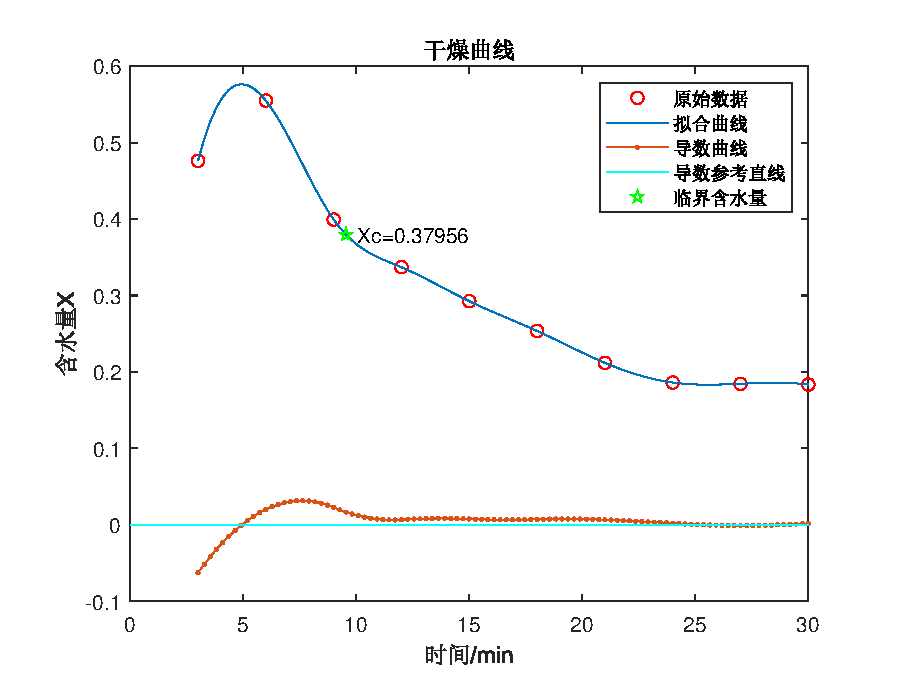
\includegraphics[width=1\textwidth]{plot.eps}
	\caption{运行示例}
\end{figure}
\newpage
\begin{lstlisting}
% 数据来自上机材料5 3.1
function exam5_3_1
t=3:3:30;
G1=[10.2 13.9 12.16 13.49 13.74 12.01 11.55 11.02 12 12.12];
G2=[6.91 8.94 8.69 10.09 10.63 9.58 9.53 9.29 10.13 10.24];
A=1.83;
X=(G1-G2)./G2;
tt=linspace(3,30);
% 插值
pp=spline(t,X);
ppv=fnval(pp,tt);
plot(t,X,'ro') %绘制原始数据,红色圆圈
hold on %保持图形窗口,继续绘制曲线
plot(tt,ppv) %绘制拟合曲线,观察插值结果
% 微分
figure %打开新图形窗
dp=fnder(pp);
dpv=-fnval(dp,tt)./A;% 干燥速率
plot(t,X,'ro',tt,ppv,tt,dpv,'.-') %同时绘制两条曲线
axisX=refline(0,0) %绘制斜率0,截距0的参考直线
axisX.Color='c'
% 计算临界含水量并标注
Um=max(dpv);
loc=find(dpv>Um/2,1,'last'); %临界含水量在向量中索引
tc=tt(loc);% 临界时间
hold on
plot(tc,ppv(loc),'gp') %临界含水量
% 图名
title('干燥曲线')
% 添加图例
legend('原始数据','拟合曲线','导数曲线','导数参考直线','临界含水量')
% 设置坐标轴
xlabel('时间/min')
ylabel('含水量X')
% 文字标注
text(tc+0.5,ppv(loc),strcat('Xc=',num2str(ppv(loc))))
\end{lstlisting}
\section{函数}
\subsection{基本用法与子函数}
\begin{lstlisting}[frame=single,numbers=left]
% 注意:[]与()的使用
function [`\mlplaceholder{y1}`,`\mlplaceholder{y2}`,..]=FunName(`\mlplaceholder{x1}`,`\mlplaceholder{x2}`,..)
%主函数下,没有输入,只有输出的子函数,如果不位于末尾,需要写end
%仅能在主函数内部调用,无法在外部调用
function y=SubFunName
\end{lstlisting}
\subsection{匿名函数}
函数$f(x,y)=x^2+y^2=-1$可表示如下:
\begin{lstlisting}[frame=single,numbers=left]
f=@(x,y) x^2+y^2-1;
f(1,2) %输出为4
\end{lstlisting}
\section{关系与逻辑运算}
\subsection{主要运算符与函数}
\textbf{关系操作符}:==、~=、>

\textbf{关系运算函数}:find()~非零元素下标
\begin{lstlisting}
a=[1 2 3];
find(a>=2) %输出为[2 3]
\end{lstlisting}

\textbf{逻辑运算}:\& (与)~~~|~(或)~~~\~{}~(非)~~~xor~(异或)
\begin{lstlisting}
a=[0 1 1];b=[0 0 1];
find(a&b) %输出为 3
\end{lstlisting}
\subsection{优先级}
\begin{figure}[htbp]
	\centering
	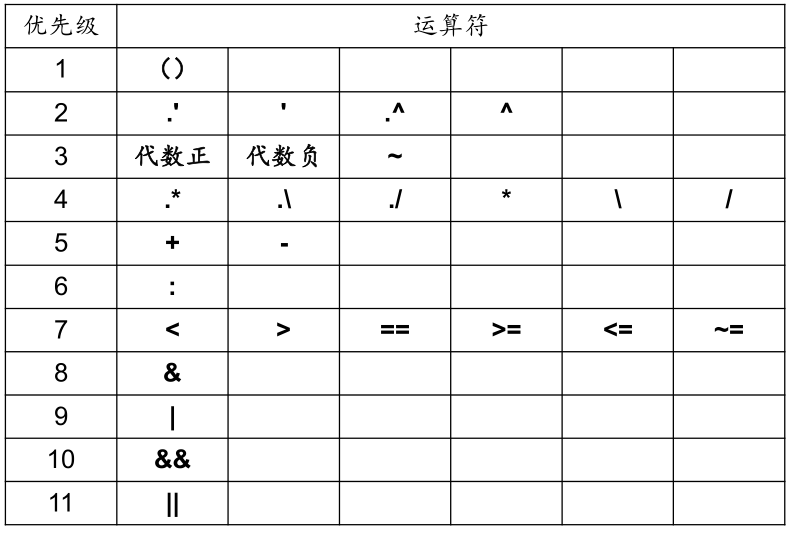
\includegraphics[width=0.6\textwidth]{priority.png}
	\caption{运算优先级}
\end{figure}
\newpage
\section{MATLAB程序控制}
\subsection{if选择语句}
\begin{lstlisting}[frame=single,numbers=left]
if `\mlplaceholder{condition1}`
    `\mlplaceholder{statements1}`
elseif `\mlplaceholder{condition2}`
    `\mlplaceholder{statements2}`
else
    `\mlplaceholder{statements3}`%譬如error(`\mlplaceholder{报错内容}`)
end
\end{lstlisting}
\subsection{for循环语句}
\begin{lstlisting}[frame=single,numbers=left]
for `\mlplaceholder{循环变量}`=`\mlplaceholder{初值}`:`\mlplaceholder{步长}`:`\mlplaceholder{终值}`
    `\mlplaceholder{循环语句}`
end
\end{lstlisting}
\subsection{whlie循环语句}
\begin{lstlisting}[frame=single,numbers=left]
while `\mlplaceholder{条件表达式}`
    `\mlplaceholder{循环语句}`
end
\end{lstlisting}
\begin{note}
了解continue、break、return函数的作用。break跳出该层循环,continue进入该层循环的下一次迭代,return退出程序或函数返回。
\end{note}
\chapter{矩阵操作与线性方程组求解}
\begin{introduction}
\item cat、repmat函数
\item 索引与下标
\item find、max、sum函数
\end{introduction}



\section{矩阵生成与性质}
\subsection{矩阵的拼接与复制}
\begin{lstlisting}[frame=single,numbers=left]
% 拼接矩阵
cat(`\mlplaceholder{DIM}`,A,B)
% 举例如下
A=[1 2];
B=[3 4];
% DIM=1,按行拼接
cat(1,A,B) %将得到[1 2 3 4]
% DIM=2,按列拼接
cat(2,A,B) %将得到[1 2;3 4]
\end{lstlisting}

\begin{lstlisting}[frame=single,numbers=left]
% 将矩阵A复制M行N列
repmat(A,`\mlplaceholder{M}`,`\mlplaceholder{N}`)
% 举例如下
A=[1 0];
repmat(A,2,3) % 将得到[1 0 1 0 1 0;1 0 1 0 1 0]
\end{lstlisting}
\subsection{常见工具矩阵}
\begin{lstlisting}[frame=single,numbers=left]
[] %空阵
zeros(n); %n阶全零阵
zeros(m,n); %m行n列全零阵
%ones用法同zeros,全1阵
\end{lstlisting}

\subsection{矩阵基本性质函数}
\begin{lstlisting}[frame=single,numbers=left]
% size函数与length函数
X=zeros(2,3);
D=size(X) %得D=[2,3],行数与列数
L=length(X) %得L=3,相当于max(size(X))
\end{lstlisting}
\section{矩阵操作与分析}
\subsection{索引与下标}
\begin{lstlisting}[frame=single,numbers=left]
% 索引
A(n) %按照(维数>)列>行的顺序标注矩阵元素
% 举例
A=[1,2,3;4,5,6];
A(1:6) %先列后行,结果为 1 4 2 5 3 6
A([end,end-1]) %结果为 6 3
\end{lstlisting}

\begin{lstlisting}[frame=single,numbers=left]
% 下标
A(m,n) %第m行第n列元素
% 举例
A=[1,2,3;4,5,6];
A(2,1) %结果为4
\end{lstlisting}

\begin{lstlisting}[frame=single,numbers=left]
% 排序
sort(A) %第m行第n列元素
% 举例
A=[1,2,3;4,5,6];
A(2,1) %结果为4
\end{lstlisting}

\subsection{逻辑与关系运算与查找}
\begin{lstlisting}[frame=single,numbers=left]
% 查找元素值
A(`\mlplaceholder{condition}`)
% 举例
A=[1,2,3;4,5,6];
A(A-2==0|A-3==0|A-4==0) %按列查找,结果为[4;2;3]
\end{lstlisting}

\begin{lstlisting}[frame=single,numbers=left]
% 查找元素索引
find(`\mlplaceholder{condition}`)
% 举例
A=[1,2,3;4,5,6];
find(A-2==0|A-3==0|A-4==0) %按列查找,结果为[2;3;5]
\end{lstlisting}

\begin{lstlisting}[frame=single,numbers=left]
% 查找元素最大值
max(A)
% 举例
A=[1,2,3;4,5,6];
max(A) %每列最大值,结果为[4 5 6]
[Rmax I]=max(A) %Rmax=[4 5 6],I=[2;2;2],返回在指定维度中的位置
\end{lstlisting}
\subsection{矩阵分析}
\begin{lstlisting}[frame=single,numbers=left]
% 求和
sum(A)
% 举例
A=[1,2,3;4,5,6];
sum(A) %按列求和,结果为[5 7 9]
sum(A,2) %按行求和,结果为[6;15]
\end{lstlisting}

\section{线性方程组的求解}
\subsection{高斯消元法}
\begin{definition}{高斯消元法}{}
基本思路为:化为上三角阵,回代求解。
\end{definition}

对于方程组
\[
AX=\emph{\textbf{b}}
\]

解可以表示为
\[
X=A\_\emph{\textbf{b}}
\]
\subsection{作答模板}
\begin{lstlisting}[frame=single,numbers=left]
% 得到所需矩阵A、b,注意对齐方式!
A=[`\mlplaceholder{系数矩阵}`];b=[`\mlplaceholder{增广矩阵}`];
% 使用左除命令求解
x=A\b;
\end{lstlisting}
\begin{problem}
假设一混合物由硝基苯$C_6H_5NO_2$、苯胺$C_6H_7N$、氨基丙酮$C_3H_7NO$和乙醇$C_2H_6O$组成。对该混合物进行元素分析,结果各元素\footnote{原子量:C为12,H为1,0为16,N为14。}的质量百分数为:$w_C=57.78\%,w_H= 7.92\%,w_N= 11.23\%,w_O= 23.07\%$。试编写一个MATLAB函数:

1)确定上面四种化合物在混合物中所占的质量百分数,采用 fprintf 函数将结果显示在屏幕上;

2) 检验求得的质量分数之和是否为 1,如果是则在屏幕上显示信息:Calculation succeed。如果否,则显示警告信息:The calculation is wrong。
\end{problem}

\begin{solution}
\begin{lstlisting}
function example2_1
N=[6 5 1 2;6 7 1 0;3 7 1 1;2 6 0 1]; %四种分子中的C、H、N、O数,顺序下同
M=[12 1 14 16];% 原子量
M=repmat(M,4,1);
A=M.*N; % 原子量之和
% 分子中,四种元素的质量分数
A(1,:)=A(1,:)/sum(A(1,:));
A(2,:)=A(2,:)/sum(A(2,:));
A(3,:)=A(3,:)/sum(A(3,:));
A(4,:)=A(4,:)/sum(A(4,:));
b=[0.5778 0.0792 0.1123 0.2307]';% 总质量分数
x=A'\b;% 关键命令!
% 两位精度显示,并自动换行
fprintf('The percentage of C6H5NO2 is %.2f%%\n',100*x(1))
fprintf('The percentage of C6H7N is %.2f%%\n',100*x(2))
fprintf('The percentage of C3H7NO is %.2f%%\n',100*x(3))
fprintf('The percentage of C2H6O is %.2f%%\n',100*x(4))
if sum(x)==1
    disp('Calculation succed')
else
    warning('The calculation is wrong')
end
\end{lstlisting}

\begin{figure}[htbp]
\centering
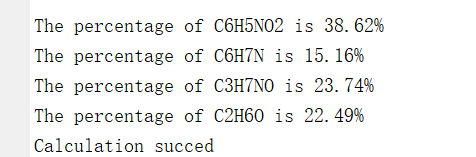
\includegraphics[width=0.5\textwidth]{exampe2_1.png}
\caption{运行结果}
\end{figure}

\end{solution}
\chapter{非线性方程(组)求解}
\begin{introduction}
\item 求解函数fzero、fslove、roots
\item 数值求解方法
\end{introduction}
\section{求解函数}\label{func}
\subsection{fzero函数}
fzero 函数是 MATLAB 里用于求解\textcolor{third}{\textbf{单个}}非线性方程的函数。它的基本使用格式如下:
\begin{lstlisting}[frame=single,numbers=left]
% 完整形式
[x,fval,exitflag,output]=fzero(fun,x0,options, p1, p2, ...)
\end{lstlisting}

\begin{lstlisting}[frame=single,numbers=left]
% 常用形式
x=fzero(`\mlplaceholder{fun}`,`\mlplaceholder{x0}`)
% 其中,`\mlplaceholder{fun}`为匿名函数或函数句柄
% `\mlplaceholder{x0}`为迭代初值,
% 也可为区间[x1,x2],函数值在端点处异号,在端点内求根
% x为x0附近的解,如有多根,则与x0选取有关
\end{lstlisting}

对于`\mlplaceholder{fun}`的使用举例如下:

\begin{lstlisting}
% 匿名函数
fun1=@(x) x-1;
fzero(fun1,0) %结果为1
\end{lstlisting}

\begin{lstlisting}
% 函数句柄
% 编写.m文件(函数文件也可)
fzero(@fun2,0) %结果为1
function y=fun2(x)
y=x-1;
end %脚本中的所有函数都必须以 'end' 结束,函数(文件)中则不需要
\end{lstlisting}

二者实现的结果类似。

\newpage
\subsection{fsolve函数}
fsolve 函数是 MATLAB 里用于求解非线性\textcolor{third}{\textbf{方程组}}的函数。它的基本使用格式如下:
\begin{lstlisting}[frame=single,numbers=left]
% 完整形式
[x,fval,exit]=fsolve(fun,x0,option)
\end{lstlisting}

对于求解方程组\footnote{摘自上机材料3}:

\[ y =
\begin{cases}
x^2+y^2-1=0\\
0.75x^3-y+0.9=0
\end{cases} \]

可新建函数文件求解:

\begin{lstlisting}
% 新建文件ExperFsolve.m
function ExperFsolve
x0=[0 0];
[x,fval,exit]=fsolve(@fun,x0)
function y=fun(x)
y=zeros(2,1);
y(1)=x(1)^2+x(2)^2-1;
y(2)=0.75*x(1)^3-x(2)+0.9;
\end{lstlisting}

也可使用匿名函数求解,二者运行结果相同:
\begin{lstlisting}
x0=[0 0]; 
f=@(x) [x(1)^2+x(2)^2-1;0.75*x(1)^3-x(2)+0.9];
[x,fval,exit]=fsolve(f,x0)
\end{lstlisting}

\begin{note}
fzero函数和fsolve函数的运行结果为初值附近的解,而非全部解。
\end{note}
\subsection{roots函数}\label{ployp}
fsolve 函数是 MATLAB 里用于求解\textcolor{third}{\textbf{多项式}}的函数。它的基本使用格式如下:
\begin{lstlisting}[frame=single,numbers=left]
r=roots(`\mlplaceholder{p}`)
% 其中`\mlplaceholder{p}`为n次多项式行向量,从高(n次)到低(0次)排列
\end{lstlisting}
譬如,求解方程$x^2-1=0$,
\begin{lstlisting}
roots([1 0 -1]) %结果为[-1;1]
\end{lstlisting}
\begin{note}
roots函数可以获得多项式的所有根。
\end{note}

\newpage
\section{常用数值求解方法}
非线性方程求数值解方法有:

\textbf{逐步扫描法,二分法,牛顿法,割线法,逆二次插值...}

\begin{definition}{二分法}{}
\textbf{[基本思想]}\\
区间逐次二等分至精度要求。

\textbf{[求解精度]}\\
可靠,只要次数足够多一定能到指定精度。

\textbf{[效率]}\\
收敛速度较慢。
\end{definition}

\begin{proposition}{收敛性对比}{}
\textbf{[牛顿法]}\\
二次收敛;收敛速度不稳定,某些条件下收敛慢或根本不收敛;导数计算不便。

\textbf{[截弦法]}\\
超线性收敛;类似牛顿法;无需计算导数。

\textbf{[逆二次插值]}\\
三点构造抛物线交坐标轴迭代;整个过程收敛速度不稳定;接近终点时迭代快。
\end{proposition}
\chapter{插值与拟合}
\begin{introduction}
\item 插值与插值函数
\item interp1,spline,pchip
\item 拟合与拟合函数
\item regress、ployfit、nlinfit
\end{introduction}
\section{插值函数的基本概念}
\subsection{插值函数}
\begin{definition}{插值函数}{}
a)插值函数$\phi(x)$近似于原函数$f(x)$
\[
y=f(x)\approx\phi(x)
\]

b)在插值点$x_i$处,插值函数值$\phi(x_i)$等于原函数值$f(x_i)$
\[
\phi(x_i)=f(x_i)=y_i
\]
\end{definition}

常见形式有:

\textbf{拉格朗日多项式插值、分段三次埃米特插值、分段三次样条插值...}
\subsection{拉格朗日插值法}
\begin{definition}{拉格朗日插值法}{}
拉格朗日n次插值多项式:
\[
P_n(x)=\sum_{i=0}^{n}{y_iL_i(x)}
\]
需要(n+1)个样本点,为了实现
\[P_n(x_i)=y_i\]
我们让基函数$L_i(x)$满足
\[L_i(x)=
\begin{cases}
1 & \text{if } x=x_i\\
0 & \text{if } x\neq x_i
\end{cases} \]
我们令
\[
L_i(x)=\prod_{\substack{j=0\\j\neq i}}^{n}\frac{x-x_j}{x_i-x_j}
\]
即为基函数定义。
\end{definition}

Lagrange插值多项式的优点在于不要求数据点是等间隔的,其缺点是数据点数不宜过大,通常不超过7个,否则计算工作量大且误差大,计算不稳定。

\begin{definition}{龙格现象}{}
当次数n增大时,部分区间上误差严重,这种现象称“龙格现象”。

[解决方法]:分段插值。
\end{definition}

\begin{note}
拉格朗日插值多项式次数高,不等于插值效果好!
\end{note}
\subsection{三次样条插值}
需要知道:区间$[a,b]$内节点$x_i$处函数值$y_i$,以及端点附近导数值等。
\begin{definition}{样条插值函数$S(x)$}{}
满足条件:

a)$S(x)$在分段区间$[x_i,x_{i+1}]$上为三次多项式

b)$S(x)$、$S'(x)$、$S''(x)$在$[a,b]$上连续

c)节点处$S(x)=y_i$

\end{definition}
\begin{note}
[自然边界条件\footnote{我的理解是:可在边界附近有较好的单调性。}]
:\quad $S''(x_0)=S''(x_n)=0$
\end{note}

\subsection{分段三次埃米特插值}
需要知道:$x_i$处的函数值$y_i$和导数值$y_i'$。
\begin{definition}{Hermite插值函数$H(x)$}{}
a)每个插值区间上H(x)为三次多项式

b)插值函数值等于节点值
\[H(x_i)=y_i
\]
c)插值函数一阶导数等于节点处导数值
\[H'(x_i)=y_i'
\]
\end{definition}

\begin{note}
二者不同之处在于一阶导数的确定方法不同。
其中,埃米特插值可保持函数形状。
\end{note}

\newpage

\section{MATLAB中的插值函数}
\subsection{interp1函数}
\begin{lstlisting}[frame=single,numbers=left]
% 调用格式
yi=interp1(x,y,xi,’`\mlplaceholder{method}`’)
% x,y为样本数据,xi为插值点
% `\mlplaceholder{method}`省略时默认线性插值
% `\mlplaceholder{method}`可选:
% 最近插值nearest、埃米特插值pchip、样条插值spline
\end{lstlisting}

\subsection{pichp函数与spline函数}\label{spline}
\begin{lstlisting}[frame=single,numbers=left]
% 调用格式
% 插值函数值
yi=pchip(x,y,xi)
% 插值函数
pp=pchip(x,y)
% spline函数使用方式相同,从略
\end{lstlisting}

以下三种调用形式结果相同:
\begin{lstlisting}[frame=single,numbers=left]
y1=interp1(x,y,xi,'pchip')
\end{lstlisting}
\begin{lstlisting}[frame=single,numbers=left]
yi=pchip(x,y,xi)
\end{lstlisting}
\begin{lstlisting}[frame=single,numbers=left]
pp=pchip(x,y);
yi=fnval(pp,xi)
\end{lstlisting}

\begin{note}
可以参考\ref{fnval}中的关于函数fnval的介绍,应用见\ref{cubic}。
\end{note}

\newpage
\section{拟合函数的基本概念}
\textcolor{third}{\textbf{拟合函数}}\textbf{不要求}函数完全通过数据点,常用方法为\textbf{最小二乘法}。

\begin{definition}{最小二乘法}{}
[原理]

近似函数在各实验点的计算结果与实验结果的偏差平方和最小。

[线性最小二乘]

可通过解方程组得到拟合函数。

[非线性最小二乘]

a)线性化;

b)直接迭代。
\end{definition}
\section{MATLAB中的拟合函数}\label{fit}
\subsection{ployfit函数}
polyfit是MATLAB的\textcolor{third}{\textbf{多项式拟合}}函数。
\begin{lstlisting}[frame=single,numbers=left]
% 调用格式
p=polyfit(x,y,n)
% x,y为样本,n为多项式次数
\end{lstlisting}

常与polyval联合使用,计算指定点的值:
\begin{lstlisting}[frame=single,numbers=left]
% 调用格式
yy=polyval(p,xx)
\end{lstlisting}

\begin{note}
此处p定义与roots函数\ref{ployp}中相同,请对照理解。
\end{note}
\subsection{regress函数}
regress是MATLAB的\textcolor{third}{\textbf{多元线性拟合 }}函数。
\begin{lstlisting}[frame=single,numbers=left]
% 调用格式
b=regress(y,x)
% n个自变量xi,进行m次实验,得到m次结果yi
% y为m行1列向量
% x为m行n列矩阵
\end{lstlisting}

\begin{note}
可以拟合线性化后的非线性函数。
\end{note}

\newpage

\begin{problem}\label{problemRegress}
已知x1=1:6,x2=1.5:0.2:2.5,y=[5.9512 10.6730 15.5676 20.6234 25.8599 31.2622]。试编写函数,采用以上数据拟合y=a*x1+b*x2+c*x1\^{}2+d*x1*x2中的系数\footnote{摘自隋志军老师课件W09}。
\end{problem}

\begin{solution}
将x1,x2,x1\^{}2和x1*x2视为自变量,则以上的拟合为多元线性拟合,可以采用regress函数求解。
\begin{lstlisting}
function LinearFitting
x1=1:6;
x2=1.5:0.2:2.5;
y=[5.9512 10.6730 15.5676 20.6234 25.8599 31.2622];
X=[x1;x2;x1.^2;x1.*x2];
% 关键函数
% 注意按照列的形式输入
b=regress(y',X') %结果为[0;1.0775;-0.5687;3.2694],即[a;b;c;d]
\end{lstlisting}

可进一步作图观察拟合结果:
\begin{lstlisting}
bb=repmat(b,1,6);
yi=sum(bb.*X);
plot(x1,y,'rp',x1,yi,'bo')
legend('原始数据','拟合数据')
\end{lstlisting}

\begin{figure}[htbp]
\centering
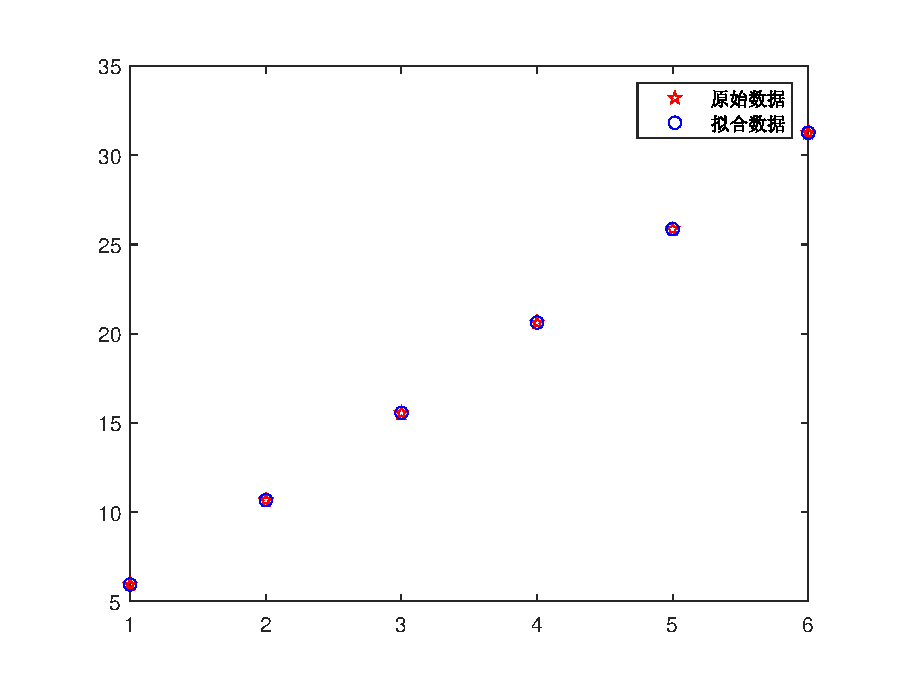
\includegraphics[width=0.8\textwidth]{regress.eps}
\caption{regress拟合效果图}
\end{figure}
\end{solution}

\newpage

\subsection{nlifit函数}
\begin{lstlisting}[frame=single,numbers=left]
beta=nlinfit(x,y,fun,beta0)
% x,y用法与regress函数类似
% fun可为匿名函数或函数句柄
% beta0是回归系数初值,beta为估计出的回归系数
\end{lstlisting}

\begin{note}
非线性方程建议采用直接非线性最小二乘法拟合,fun调用可参考\ref{func}。
\end{note}

\begin{problem}
用nlifit函数求解例题\ref{problemRegress}:
\end{problem}

\begin{solution}
\begin{lstlisting}
function NonLinearFitting
x1=1:6;
x2=1.5:0.2:2.5;
y=[5.9512 10.6730 15.5676 20.6234 25.8599 31.2622];
beta0=[0 0 0 0];%对结果影响较大
% 关键函数
beta=nlinfit([x1',x2'],y',@fun,beta0) %与初值选取有关
% 验证结果
yi=fun(beta,[x1',x2']); %拟合函数在样本处点的函数值
plot(x2,y,'ro',x2',yi,'bp') %作图对比
errMax=max(abs(y'-yi)) %最大偏差为0.0034,与regress相同

%拟合函数部分
function y=fun(Beta,x)
a=Beta(1);b=Beta(2);c=Beta(3);d=Beta(4); %提高代码可读性
x1=x(:,1);x2=x(:,2); %与上一行本质上可以略去,不过下一行会比较复杂
y=a*x1+b*x2+c*x1.^2+d*x1.*x2;
\end{lstlisting}
\end{solution}
\newpage
\subsection{csaps函数}\label{fnval}
\begin{lstlisting}[frame=single,numbers=left]
% Cubic smoothing spline 平滑三次样条拟合函数
% 拟合函数
pp=csaps(x,y,p,[],w)
% p:平滑参数,范围[0,1],默认为1,即spline
% w:误差权重,默认为1
% 拟合函数值
values=csaps(x,y,p,xx,w)
\end{lstlisting}

\begin{lstlisting}[frame=single,numbers=left]
pp=csaps(x,y,p,[],w);
values=fnval(pp,xx) 
% 函数fnval
fnval(f,x) %计算函数f在x处的函数值
\end{lstlisting}

\begin{note}
可以参考\ref{spline}中的相关介绍。
\end{note}
\chapter{数值微分与积分}
\begin{introduction}
\item 数值微分的三种思路
\item diff与fnder函数
\item 插值型积分公式
\item quad与quadl函数
\end{introduction}
\section{数值微分}
\subsection{建立数值微分公式}
\begin{definition}{三种思路}{}
[差分]

从微分定义出发,通过近似处理,得到数值微分的近似公式。

[插值]

从插值近似公式出发,对插值公式的近似求导可得到数值微分的近似公式。

[拟合]

先用最小二乘拟合方法根据已知数据或得近似函数(如样条函数),再对此近似函数求微分可得到数值微分的近似公式。
\end{definition}
\subsection{向前差分及diff函数}
在MATLAB中,可用diff求向量相邻元素的差值:
\begin{lstlisting}[frame=single,numbers=left]
% 向前差分函数diff
% 调用形式
Y=diff(X,n,dim)
% X:输入矩阵
% n:差分阶数,默认1
% dim:行1列2,默认按行差分
% Y=diff(X,2)等价于Y=diff(diff(X))
\end{lstlisting}

\begin{lstlisting}[frame=single,numbers=left]
% 常用形式
Y=diff(X)
% 若X为m阶向量,则上式等价于
Y=[X(2)-X(1) X(3)-X(2)..X(m)-X(m-1)]
\end{lstlisting}

\newpage

则可用\textcolor{third}{\textbf{一阶向前差分}}近似计算$\frac{\mathrm{d}x}{\mathrm{d}y}$。
\begin{lstlisting}[frame=single,numbers=left]
diff(y)./diff(x)
\end{lstlisting}



\subsection{三次插值与fnder函数}\label{cubic}
\begin{note}
关于spline/phchip的函数介绍见\ref{spline},不再赘述。
\end{note}

解决该类问题需要用到fnder函数,介绍如下:

\begin{lstlisting}[frame=single,numbers=left]
% Differentiate function
% 调用格式
fprime=fnder(f,dorder) %dorder求导阶数,默认为1
\end{lstlisting}
\begin{lstlisting}[frame=single,numbers=left]
% 常用形式
pp=spline(x,y); %pp为三次样条插值函数
fprime=fnder(pp); %fprime为pp的一阶导函数
value=fnval(fprime,x) %计算在x处的导数值
\end{lstlisting}

\subsection{拟合与微分}\label{fitd}
\begin{note}
此节\ref{fitd}隋志军老师于考试要点W12中未作要求,部分内容可参考拟合章节\ref{fit}。
\end{note}

\begin{lstlisting}[frame=single,numbers=left]
% 多项式拟合求微分
p=ployfit(x,y,n); %多项式向量
dp=polyder(p); %多项式导函数
dpv=ployval(dp,x); %计算函数值,也可用fnval(dp,x)
\end{lstlisting}

\begin{lstlisting}[frame=single,numbers=left]
% 样条拟合求微分
% 可用cspas/spaps/spap2
% 举cspas为例:
pp=csaps(x,y); %pp为样条拟合函数
fprime=fnder(pp); %fprime为pp的一阶导函数
value=fnval(fprime,x) %计算在x处的导数值
\end{lstlisting}
\section{数值积分}
\subsection{基本思路与方法}
基本思路来自于\textcolor{third}{\textbf{插值法}}, 通过构造一个插值多项式$Pn(x)$作为$f(x)$的近似表达式,用$Pn(x)$的积分值作为$f(x)$的近似积分值。
\begin{definition}{Newton-Cotes求积公式}{}
a)等距节点,分为n份;

b)使用Lagrange插值多项式近似。
\end{definition}
特别地,改变其中等分数n=1,2,可得:
\begin{enumerate}
  \item \textbf{梯形求积公式};
  \item \textbf{Simpson求积公式}。
\end{enumerate}

\begin{definition}{复化求积}{}
a)将积分区间$[a,b]$分为n个相等子区间;

b)对每个子区间使用梯形求积或Simpson求积公式。
\end{definition}

\begin{definition}{自适应求积}{}
a)考虑区间上及其二等分以后的两个Simpson积分和,分别记为S1、S2;

b)~S1、S2满足精度要求则不再二等分,取该区间积分值为S2。

[注]:可以不等步长。
\end{definition}

\begin{note}
牛顿-科特斯和高斯-勒让德求积公式,从略。
\end{note}

\subsection{quad和quadl函数}
自适应Simpson法数值积分:\textcolor{third}{\textbf{quad}}。

\begin{lstlisting}[frame=single,numbers=left]
% 调用形式
q=quad(fun,a,b,tol,trace,p1,p2,…)
% fun 被积函数
% a,b 积分上下限
% tol 求解精度
\end{lstlisting}

\begin{lstlisting}[frame=single,numbers=left]
% 常用形式
q=quad(fun,a,b)
\end{lstlisting}
自适应Lobatto数值积分:\textcolor{third}{\textbf{quadl}},结果更精确。
\begin{lstlisting}[frame=single,numbers=left]
% quadl函数与quad函数的使用完全一致
q=quadl(fun,a,b)
q=quadl(fun,a,b,tol,trace,p1,p2,…)
\end{lstlisting}

\begin{note}
被积函数支持向量化运算,函数表达式 中的必须使用点运算符号!
\end{note}

\begin{note}
fun用法请参考\ref{func}。
\end{note}

\chapter{常微分方程数值解}
\begin{introduction}
\item 定义与分类
\item 数值解方法
\item MATLAB中微分方程的表示方法
\item ode45函数
\end{introduction}
\section{常微分方程}
\subsection{定义}
含有未知函数导数的方程。
\subsection{分类}
分为\textbf{初值问题}与\textbf{边值问题}。

本节主要关注利用\textbf{步进法}解决\textbf{初值问题}。
\subsection{初值问题的数值解方法}
\begin{itemize}
	\item 欧拉法:单步,矩形公式;
	\item 龙格-库塔法:单步,线性组合;
	\item 阿达姆斯法:多步。
\end{itemize}
\section{MATLAB解常微分方程}
\subsection{微分方程的表示}
对于\textcolor{third}{\textbf{微分方程}}:
\[y'=2x+y\]
\begin{lstlisting}[frame=single,numbers=left]
% 可表示为
function dy=odefun(x,y)
dy=2*x+y

% 或
odefun=@(x,y) 2*x+y
\end{lstlisting}

对于\textcolor{third}{\textbf{微分方程组}}:
\[
\begin{cases}
y_1'=y_1-y_2+x\\
y_2'=y_1'+y_2
\end{cases} \]

\begin{lstlisting}[frame=single,numbers=left]
% 可表示为
function dy=odefun(x,y)
dy1=y(1)-y(2)+x;
dy2=dy1+y(2);
dy=[dy1;dy2]; %方程组的dy用列向量输出!
\end{lstlisting}

对于\textcolor{third}{\textbf{高阶微分方程组}}:
\[
\begin{cases}
y_1'=xy_2'+y_1\\
y_2''=y_1'+sin(x)y_2
\end{cases} \]

\begin{lstlisting}[frame=single,numbers=left]
% 变量代换
% 令y(1)=y1,y(2)=y2,y(3)=y2'
% 可表示为
function dy=odefun(x,y)
dy1=0;dy2=0;ddy2=0;
dy1=x*ddy2+y1;
dy2=y(3);
ddy2=dy1+sin(x)*y(2);
dy=[dy1;dy2;ddy2];
\end{lstlisting}

\subsection{ode45函数}
\begin{lstlisting}[frame=single,numbers=left]
% 常用形式
[T,Y]=ode45(fun,TSPAN,Y0)% TSPAN 求解区间;Y0 初值
% 带参数
[T,Y]=ode45(fun,TSPAN,Y0,options)
% 常用求解参数
%输出T与Y的关系图,类似plot(T,Y)
options=odeset(‘outputfcn’,‘odeplot’) 
%输出求解变量Y之间的二维相平面图,类似plot(Y(2),Y(2))
options=odeset('outputfcn','odephas2') 
\end{lstlisting}

\newpage
\begin{problem}
某串联反应各物质的浓度与反应时间 $t$ 的关系如下\footnote{改自隋志军老师“课程练习题”}:
\[
	\begin{cases}
		\frac{\dd{C_{A}}}{\dd{t}} = - k_{1} C_{A} \\
		\frac{\dd{C_{B}}}{\dd{t}} = k_{1} C_{A} - k_{2} C_{B} \\
		\frac{\dd{C_{C}}}{\dd{t}} = k_{2} C_{B} - k_{2} C_{C} \\
		\frac{\dd{C_{D}}}{\dd{t}} = k_{3} C_{C} - k_{4} C_{D} \\
		\frac{\dd{C_{E}}}{\dd{t}} = k_{4} C_{D}
	\end{cases}
\]
\begin{figure}[htbp]
\centering
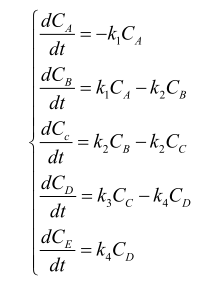
\includegraphics[width=0.4\textwidth]{ode.png}
\end{figure}
\\已知 $k_{1} = 0.04$,$k_{2}=0.05$,$k_{3}=0.10$,$k_{4}=0.08$,反应开始时只有 A 存在,其浓度为 1。
试编写一个 MATLAB 函数,求前 \SI{60}{s} 中每隔 \SI{5}{s} 时各物质的浓度,并作图。
\end{problem}

\begin{solution}

\begin{lstlisting}
function solveC
T=0:5:60;
C0=[1 0 0 0 0];
% 设置图形输出
options=odeset('outputfcn','odeplot');
% 核心函数
[T C]=ode45(@odefun,T,C0,options);
% 常微分方程组
function dC=odefun(T,C)
k1=0.04;k2=0.05;k3=0.10;k4=0.08;
dCA=-k1*C(1);
dCB=k1*C(1)-k2*C(2);
dCC=k2*C(2)-k2*C(3);
dCD=k3*C(3)-k4*C(4);
dCE=k4*C(4);
dC=[dCA;dCB;dCC;dCD;dCE]; %按列
\end{lstlisting}

\end{solution}





%\include{end} 
%\chapter{MWE}

%% 代码环境
%引入函数时用
\begin{lstlisting}[frame=single,numbers=left]
`\mlplaceholder{x}`
\end{lstlisting}

%例题时用
\begin{lstlisting}
\end{lstlisting}

%-------------------------------------------

%% 其他

%问题与解答
\begin{problem}
\end{problem}

\begin{solution}
\end{solution}

%插入图片
\begin{figure}[htbp]
\centering
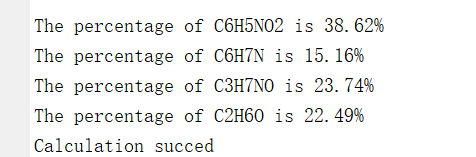
\includegraphics[width=0.7\textwidth]{exampe2_1.png}
\caption{}
\end{figure}

%插入定义
\begin{definition}{}{}
\[\]
\end{definition}

%插入提示
\begin{note}
拉格朗日插值多项式次数高,不等于插值效果好!
\end{note}

%加粗变色
\textcolor{third}{\textbf{方程组}}

%引用
\ref{func} %模板
%-------------------------------------------
\end{document}
